\usetikzlibrary{calc}


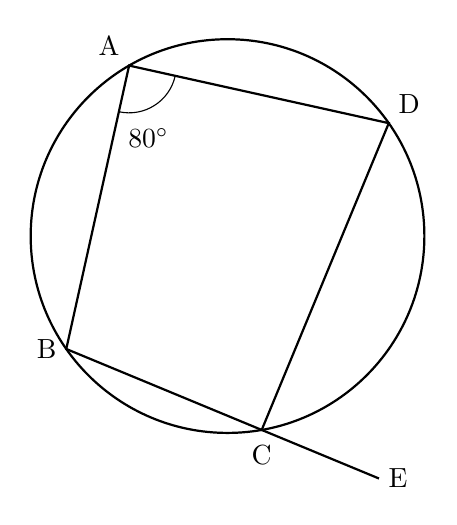
\begin{tikzpicture}[scale=1]

    % --- Coordinates ---
    % Center of the circle (origin)
    \coordinate (O) at (0,0);
    
    % Defining vertex coordinates on the circumference (radius 2.5cm)
    % C is moved further left (280 degrees) to match the visual proportions
    \coordinate (A) at (120:2.5);  % Vertex A (Top Left)
    \coordinate (B) at (215:2.5);  % Vertex B (Bottom Left)
    \coordinate (C) at (280:2.5);  % Vertex C (Bottom Left-Center)
    \coordinate (D) at (35:2.5);   % Vertex D (Top Right)
    
    % Point E is defined as an extension of the line BC to ensure collinearity
    \coordinate (E) at ($(B)!1.6!(C)$);

    % --- Drawing Main Geometry ---
    % Drawing the circumscribed circle
    \draw[thick] (O) circle (2.5);
    
    % Drawing the inscribed cyclic quadrilateral ABCD
    \draw[thick] (A) -- (B) -- (C) -- (D) -- cycle;
    
    % Drawing the extension line from C to E (Collinear with B and C)
    \draw[thick] (C) -- (E);

    % --- Angles and Measurements ---
    % FIXED ARC: Calculated to span exactly between sides AB and AD
    % Start angle -102.5 (aligns with AB) to -12.5 (aligns with AD)
    \draw (A) +(-102.5:0.6) arc (-102.5:-12.5:0.6);
    
    % Placing the angle label 80°
    \node at ($(A) + (-75:0.95)$) {$80^{\circ}$};

    % --- Point Labels ---
    % Labels positioned to mirror Figure 9
    \node[above left] at (A) {A};
    \node[left] at (B) {B};
    \node[below=2pt] at (C) {C};
    \node[above right] at (D) {D};
    \node[right] at (E) {E};

\end{tikzpicture}